\documentclass[10pt]{beamer}\usepackage[]{graphicx}\usepackage[]{color}
%% maxwidth is the original width if it is less than linewidth
%% otherwise use linewidth (to make sure the graphics do not exceed the margin)
\makeatletter
\def\maxwidth{ %
  \ifdim\Gin@nat@width>\linewidth
    \linewidth
  \else
    \Gin@nat@width
  \fi
}
\makeatother

\definecolor{fgcolor}{rgb}{0.345, 0.345, 0.345}
\newcommand{\hlnum}[1]{\textcolor[rgb]{0.686,0.059,0.569}{#1}}%
\newcommand{\hlstr}[1]{\textcolor[rgb]{0.192,0.494,0.8}{#1}}%
\newcommand{\hlcom}[1]{\textcolor[rgb]{0.678,0.584,0.686}{\textit{#1}}}%
\newcommand{\hlopt}[1]{\textcolor[rgb]{0,0,0}{#1}}%
\newcommand{\hlstd}[1]{\textcolor[rgb]{0.345,0.345,0.345}{#1}}%
\newcommand{\hlkwa}[1]{\textcolor[rgb]{0.161,0.373,0.58}{\textbf{#1}}}%
\newcommand{\hlkwb}[1]{\textcolor[rgb]{0.69,0.353,0.396}{#1}}%
\newcommand{\hlkwc}[1]{\textcolor[rgb]{0.333,0.667,0.333}{#1}}%
\newcommand{\hlkwd}[1]{\textcolor[rgb]{0.737,0.353,0.396}{\textbf{#1}}}%
\let\hlipl\hlkwb

\usepackage{framed}
\makeatletter
\newenvironment{kframe}{%
 \def\at@end@of@kframe{}%
 \ifinner\ifhmode%
  \def\at@end@of@kframe{\end{minipage}}%
  \begin{minipage}{\columnwidth}%
 \fi\fi%
 \def\FrameCommand##1{\hskip\@totalleftmargin \hskip-\fboxsep
 \colorbox{shadecolor}{##1}\hskip-\fboxsep
     % There is no \\@totalrightmargin, so:
     \hskip-\linewidth \hskip-\@totalleftmargin \hskip\columnwidth}%
 \MakeFramed {\advance\hsize-\width
   \@totalleftmargin\z@ \linewidth\hsize
   \@setminipage}}%
 {\par\unskip\endMakeFramed%
 \at@end@of@kframe}
\makeatother

\definecolor{shadecolor}{rgb}{.97, .97, .97}
\definecolor{messagecolor}{rgb}{0, 0, 0}
\definecolor{warningcolor}{rgb}{1, 0, 1}
\definecolor{errorcolor}{rgb}{1, 0, 0}
\newenvironment{knitrout}{}{} % an empty environment to be redefined in TeX

\usepackage{alltt}
\usepackage{amsmath}
\usepackage{amssymb}
\usepackage{geometry}
\usepackage{graphicx}
\usepackage{url}
\usepackage{bm}

\makeatletter
\let \@sverbatim \@verbatim
\def \@verbatim {\@sverbatim \verbatimplus}
{\catcode`'=13 \gdef \verbatimplus{\catcode`'=13 \chardef '=13 }} 
\makeatother

\newcommand{\SST}{\text{SST}}
\newcommand{\RSS}{\text{RSS}}
\newcommand{\SSreg}{\text{SSreg}}
\newcommand{\se}{\text{se}}
\newcommand{\reduced}{\text{reduced}}
\newcommand{\full}{\text{full}}
\newcommand{\df}{\text{df}}
\IfFileExists{upquote.sty}{\usepackage{upquote}}{}
\begin{document}

% --------------------------------------------
\begin{frame}
\large
Lecture 11:\\ 
F-test\\
STAT 632, Spring 2020\\
\end{frame}


% --------------------------------------------
\begin{frame}{Test of all the predictors}
Is there a relationship between the response variable and at least one predictor in the multiple linear regression model?\\
$$Y = \beta_0 + \beta_1 x_1 + \cdots \beta_p x_p + e$$
\vspace{5pt}

The null and alternative hypothesis for the test can be written as\\
\vspace{5pt}
$H_0: \beta_1 = \beta_2 = \cdots = \beta_p = 0$\\
There is no relationship between $Y$ and the predictor variables.\\
\vspace{7pt}
$H_A$:  at least one $\beta_j \neq 0$\\
There is a relationship between $Y$ and at least one of the predictor variables.
%When we reject $H_0$, this does not mean the full model is the best.  We do not know whether all the predictors are requires, or just a subset of them.  Predictors may also be added, transformed, or recombined.  The F-test is just the beginning.  
\end{frame}

% --------------------------------------------
\begin{frame}{Test of all the predictors}
$H_0: \beta_1 = \beta_2 = \cdots = \beta_p = 0$\\
\vspace{5pt}
$H_A$:  at least one $\beta_j \neq 0$\\
\vspace{10pt}
Test statistic:
\begin{align*}
F = \frac{(\SST - \RSS)/p}{\RSS / (n-p-1)} = 
\frac{\SSreg / p}{\RSS / (n-p-1)}
\end{align*}

\begin{itemize}
\item $\SST = \sum_{i=1}^n (y_i - \bar{y})^2$ is the total sum of squares
\item $\RSS = \sum_{i=1}^n (y_i - \hat{y}_i)^2$ is the residual sum of squares
\item $\SSreg = \sum_{i=1}^n (\hat{y}_i - \bar{y})^2$ is the regression sum of squares
\item SST = SSreg + RSS
\item $n$ is the number of observations in the data set, and $p$ is the number of predictor variables.
\end{itemize}
\end{frame}

% --------------------------------------------
\begin{frame}{Test of all the predictors}
Analysis of variance table:\\

\begin{table}
\begin{tabular}{lllll}
\hline
Source & df & Sum of Squares & Mean Square & F\\
\hline
Regression & $p$ & SSreg & $\SSreg/p$ & $\frac{\SSreg / p}{\RSS / (n-p-1)}$\\
Residual & $n-p-1$ & RSS & $\RSS/(n-p-1)$ & \\
\hline
Total & $n-1$ & SST & &\\ 
\end{tabular}
\end{table}

Most computer packages will provide some version of this table.  Ronald Fisher, the creator of the table, once said it's ``nothing but a convenient way of arranging arithmetic."  That was in 1931, when he had to all the calculations by hand.\\
\end{frame}

% --------------------------------------------
\begin{frame}{Example: NY Housing Data}
\begin{itemize}
\item Data set on housing prices from Canton, NY (scraped from Zillow.com)
\vspace{5pt}
\item The response variable is \texttt{Price} (in thousands of dollars)
\vspace{5pt}
\item The predictors
\begin{itemize}
\item \texttt{Beds}: number of bedrooms
\item \texttt{Baths}: number of bathrooms
\item \texttt{Size}: floor area of house (in thousands of square feet)
\item \texttt{Lot}: size of the lot (in acres)
\end{itemize}
\end{itemize}
\end{frame}

% --------------------------------------------
\begin{frame}[fragile]
\small
\begin{verbatim}
> library(Stat2Data)

> data(HousesNY)

> dim(HousesNY)
[1] 53  5

> head(HousesNY)
  Price Beds Baths  Size  Lot
1  57.6    3     2 0.960 1.30
2 120.0    6     2 2.786 0.23
3 150.0    4     2 1.704 0.27
4 143.0    3     2 1.200 0.80
5  92.5    3     1 1.329 0.42
6  50.0    2     1 0.974 0.34
\end{verbatim}
\end{frame}

% --------------------------------------------
\begin{frame}[fragile]
\small
\begin{verbatim}
> pairs(Price ~ Beds + Baths + Size + Lot, data=HousesNY)
\end{verbatim}
\vspace{-0.75cm}
\begin{figure}
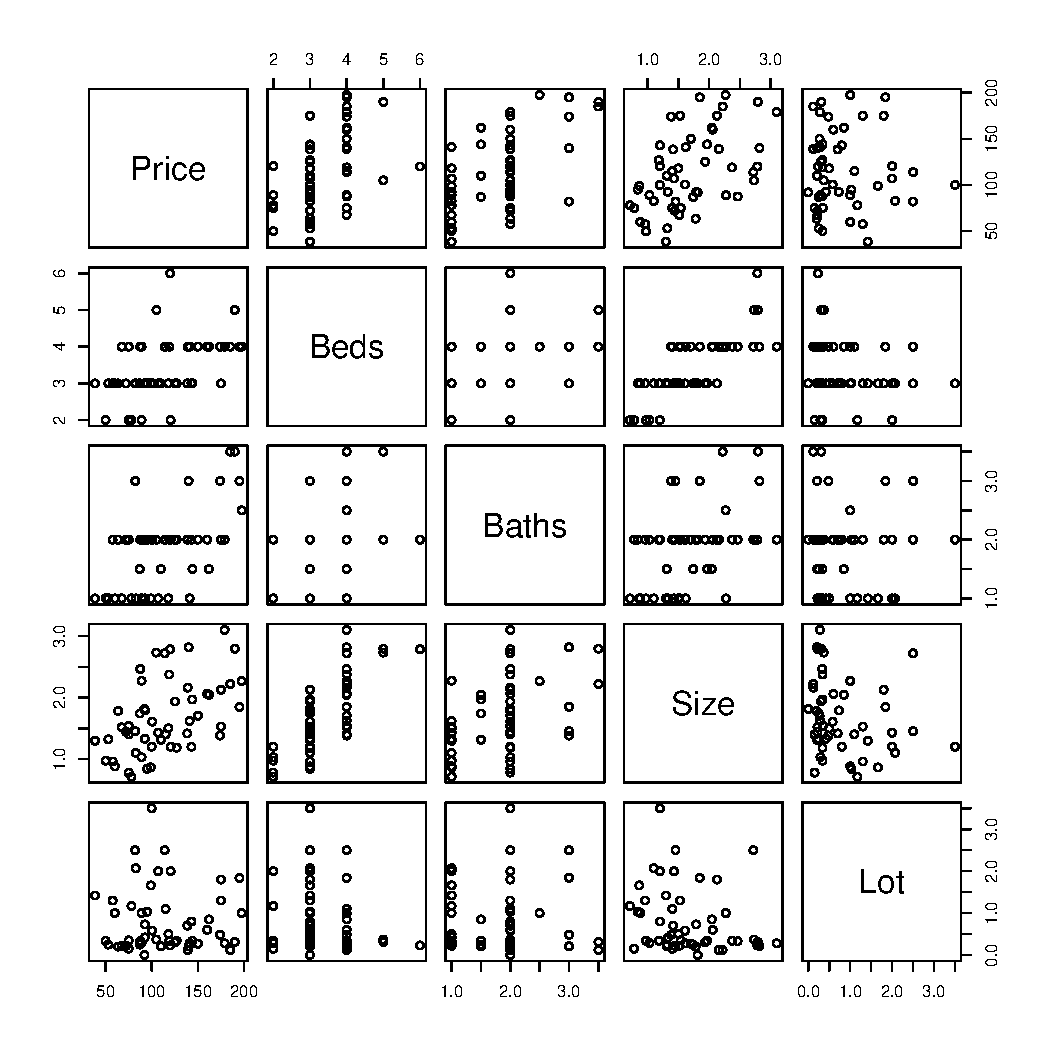
\includegraphics[scale=0.45]{figure/ny_pairs.pdf}
\end{figure}
\end{frame}

% --------------------------------------------
\begin{frame}{Example}
$H_0: \beta_1 = \beta_2 = \beta_3 = \beta_4 = 0$\\
$H_A:$ at least one $\beta_j \neq 0$\\
\vspace{10pt}

For the F-test we are comparing the full model, with all the predictors, to the null model, with no predictors.\\
\vspace{10pt}

Full model:\\
$\texttt{Price} = \beta_0 + \beta_1 \texttt{Beds} + \beta_2 \texttt{Baths} + \beta_3 \texttt{Size} + \beta_4 \texttt{Lot} + e$\\
\vspace{10pt}

Null (reduced) model:\\
$\texttt{Price} = \beta_0 + e$\\
\end{frame}

% --------------------------------------------
\begin{frame}[fragile]
\small
\begin{verbatim}
> lm_full <- lm(Price ~ Beds + Baths + Size + Lot, data=HousesNY)
> lm_null <- lm(Price ~ 1, data=HousesNY)

> anova(lm_null, lm_full)
Analysis of Variance Table

Model 1: Price ~ 1
Model 2: Price ~ Beds + Baths + Size + Lot
  Res.Df   RSS Df Sum of Sq      F   Pr(>F)    
1     52 89255                                 
2     48 52358  4     36897 8.4566 3.01e-05 ***
---
Signif. codes:  0 ‘***’ 0.001 ‘**’ 0.01 ‘*’ 0.05 ‘.’ 0.1 ‘ ’ 1
\end{verbatim}

\normalsize
Since the $p$-value $<0.001$ we reject the null hypothesis that $\beta_1 = \cdots = \beta_4 =0$.  Thus, we conclude, that at least one predictor is associated with \texttt{Price}.
\end{frame}

% --------------------------------------------
\begin{frame}[fragile]
The results of the F-test are also provided in the \texttt{summary()} output.\\
\small
\begin{verbatim}
> summary(lm_full)

Coefficients:
            Estimate Std. Error t value Pr(>|t|)   
(Intercept)   14.590     23.266   0.627   0.5336   
Beds           2.771      8.730   0.317   0.7523   
Baths         26.238      7.844   3.345   0.0016 **
Size          22.155     11.931   1.857   0.0695 . 
Lot            4.621      6.184   0.747   0.4585   
---
Signif. codes:  0 ‘***’ 0.001 ‘**’ 0.01 ‘*’ 0.05 ‘.’ 0.1 ‘ ’ 1

Residual standard error: 33.03 on 48 degrees of freedom
Multiple R-squared:  0.4134,	Adjusted R-squared:  0.3645 
F-statistic: 8.457 on 4 and 48 DF,  p-value: 3.01e-05
\end{verbatim}
\end{frame}

% --------------------------------------------
\begin{frame}[fragile]
Just for verification, we can also directly calculate the F-test statistic using the formula.
\begin{verbatim}
> n <- nrow(HousesNY)
> p <- 4
> rss <- sum(resid(lm_full)^2); rss
[1] 52357.9
> sst <- sum(resid(lm_null)^2); sst
[1] 89255.4
> fstat <- ((sst - rss) / p) / (rss / (n-p-1))
> fstat
[1] 8.456603
> 1 - pf(fstat, df1=p, df2=n-p-1)
[1] 3.0104e-05
\end{verbatim}
\end{frame}

% --------------------------------------------
\begin{frame}{Testing just one predictor}
Can one particular predictor be dropped from the model?\\
\vspace{10pt}

To test whether the coefficient for a single predictor is 0 we can either use a t-test or F-test (the results are equivalent).  In R, the t-test is less work, since the results are provided in the regression summary output.\\
\vspace{10pt}

$H_0: \beta_j = 0$\\
$H_A: \beta_j \neq 0$\\
\vspace{10pt}

Test statistic:
\begin{align*}
T_j = \frac{\hat{\beta}_j}{\se (\hat{\beta}_j)};
\quad \text{df}=n-p-1
\end{align*}
\end{frame}

% --------------------------------------------
\begin{frame}[fragile]{Example}
The regression summary in a previous slide shows that \texttt{Beds} is not significant, and can be dropped from the model, since $t=0.317$ with a $p$-value$=0.7523$.  Using the F-test we obtain the same result:\\

\small
\begin{verbatim}
> lm_full <- lm(Price ~ Beds + Baths + Size + Lot, data=HousesNY) 
> lm1 <- lm(Price ~ Baths + Size + Lot, data=HousesNY) 
> anova(lm1, lm_full)
Analysis of Variance Table

Model 1: Price ~ Baths + Size + Lot
Model 2: Price ~ Beds + Baths + Size + Lot
  Res.Df   RSS Df Sum of Sq      F Pr(>F)
1     49 52468                           
2     48 52358  1    109.87 0.1007 0.7523
\end{verbatim}
\normalsize
Notice that the $p$-values from the F-test and t-test are exactly the same.
\end{frame}

% --------------------------------------------
\begin{frame}{Testing a subset of predictors}
Suppose we want to test whether a specified subset of predictors have regression coefficients equal to 0.  This is often called the \textbf{partial F-test}.\\
\vspace{10pt}
For example, using the NY housing data, the full model is given by\\
$\texttt{Price} = \beta_0 + \beta_1 \texttt{Beds} + \beta_2 \texttt{Baths} + \beta_3 \texttt{Size} + \beta_4 \texttt{Lot} + e$\\
\vspace{10pt}
Suppose we want to test whether the coefficients for \texttt{Beds} and \texttt{Lot} are both zero.  The null and alternative hypothesis can be written as:\\
$H_0$: $\beta_1 = \beta_4 = 0$\\
$H_A$: $\beta_1 \neq 0$ or $\beta_4 \neq 0$
\end{frame}

% --------------------------------------------
\begin{frame}{Testing a subset of predictors}
For the partial F-test we use the following test statistic:\\

\begin{align*}
F = \frac{(\RSS_{\reduced} - \RSS_{\full}) / k}{\RSS_{\full} / (n-p-1)}
\end{align*}

\begin{itemize}
\item $\RSS_{\full}$ is the residuals sum of squares for the model with the full set of $p$ predictors.
\item $\RSS_{\reduced}$ is the residuals sum of squares for the reduced model with $k$ predictors removed.
\end{itemize}
\end{frame}

% --------------------------------------------
\begin{frame}[fragile]{Example}
\small
\begin{verbatim}
> lm_full <- lm(Price ~ Beds + Baths + Size + Lot, data=HousesNY)
> lm2 <- lm(Price ~ Baths + Size, data=HousesNY)
> anova(lm2, lm_full)
Analysis of Variance Table

Model 1: Price ~ Baths + Size
Model 2: Price ~ Beds + Baths + Size + Lot
  Res.Df   RSS Df Sum of Sq      F Pr(>F)
1     50 53039                           
2     48 52358  2    680.81 0.3121 0.7334
\end{verbatim}
\normalsize
The $p$-value = 0.73 is large, so we do not reject the null hypothesis that $H_0: \beta_1 = \beta_4 = 0$.  So we can remove both predictors, \texttt{Beds} and \texttt{Lot}, from the model. 
\end{frame}



% --------------------------------------------
\begin{frame}[fragile]
The $R^2$ for the full and reduced models are about the same, and the adjusted $R^2$ for the reduced model is a little higher.  This agrees with the conclusion of the F-test.  So the adjusted-R$^2$ also indicates that we can remove  \texttt{Beds} and \texttt{Lot}.
\small
\begin{verbatim}
> s1 <- summary(lm_full)
> s2 <- summary(lm2)
> 
> s1$r.squared
[1] 0.4133924
> s2$r.squared
[1] 0.4057647
> 
> s1$adj.r.squared
[1] 0.3645084
> s2$adj.r.squared
[1] 0.3819953
\end{verbatim}
\end{frame}

% --------------------------------------------
\begin{frame}[fragile]
\small
\begin{verbatim}
> summary(lm2)
Coefficients:
            Estimate Std. Error t value Pr(>|t|)   
(Intercept)   24.641     15.890   1.551  0.12728   
Baths         26.755      7.699   3.475  0.00107 **
Size          23.399      8.317   2.813  0.00699 **
---
Signif. codes:  0 ‘***’ 0.001 ‘**’ 0.01 ‘*’ 0.05 ‘.’ 0.1 ‘ ’ 1

Residual standard error: 32.57 on 50 degrees of freedom
Multiple R-squared:  0.4058,	Adjusted R-squared:  0.382 
F-statistic: 17.07 on 2 and 50 DF,  p-value: 2.233e-06
\end{verbatim}
\end{frame}

\begin{frame}{Your turn}
\vspace{-2.5cm}
Using the NY housing data, the full model is given by\\
$\texttt{Price} = \beta_0 + \beta_1 \texttt{Beds} + \beta_2 \texttt{Baths} + \beta_3 \texttt{Size} + \beta_4 \texttt{Lot} + e$\\
\vspace{10pt}
In R, conduct a partial F-test for the following hypotheses:\\
$H_0: \beta_1 = \beta_2 = \beta_4 = 0$\\
$H_A: \beta_1 \neq 0$ or $\beta_2 \neq 0$ or $\beta_4 \neq 0$\\
\vspace{10pt}
What is the $p$-value and your conclusion? 
\end{frame}

% --------------------------------------------
\begin{frame}{Summary}
\begin{itemize}
\item Use the overall F-test to test whether there is a relationship between the response and at least one predictor in the model.
\vspace{10pt}

\item Use the partial F-test to test whether there is a relationship between the response and a specified subset of two or more predictors in the model.
\vspace{10pt}

\item Use a t-test to test whether there is a relationship between the response and a single predictor in the model.
\end{itemize}
\end{frame}

\end{document}
